En el momento que sigue en la simulación, la porción de la energía cinética de la gráfica circular crece, entonces:

\begin{minipage}{0.3\textwidth}
    \begin{figure}[H]
        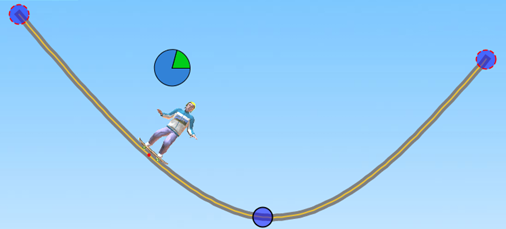
\includegraphics[width=\linewidth]{../images/q028c}
    \end{figure}
\end{minipage}\hfill
\begin{minipage}{0.6\textwidth}
    \begin{choices}
        \choice La porción de la Energía potencial permanece igual
        \choice La porción de la Energía potencial también crece
        \choice La porción de la Energía potencial disminuye
        \choice No hay manera de saberlo
    \end{choices}
\end{minipage}
